\section{Алгоритм пошуку маршруту з врахуванням розкладу руху}
\label{sec:clients-analysis}

Пошук найкоротших маршрутів з урахуванням розкладу є важливим аспектом планування та оптимізації перевезень. Він передбачає врахування часових обмежень та інформації про розклад для визначення найефективніших шляхів між пунктами. У цьому контексті алгоритм Єна в поєднанні з даними розкладу пропонує потужний підхід для вирішення цієї задачі.

Алгоритм Єна, відомий завдяки знаходженню K-найкоротших шляхів, може бути розширений для врахування обмежень розкладу. Інтегруючи інформацію про розклад в алгоритм, стає можливим визначити маршрути, які не тільки мінімізують відстань, але й враховують час прибуття та відправлення, час очікування та інші фактори, пов'язані з часом.

Пошук найкоротших маршрутів з урахуванням розкладу за допомогою алгоритму Єна відбувається в кілька етапів. По-перше, дані розкладу, які включають час прибуття і відправлення для кожної зупинки транспортної мережі, необхідно включити в графічне представлення. Це передбачає асоціювання відповідних значень часу з ребрами, що з'єднують вузли (зупинки) на графі.

Далі до модифікованого графа застосовується алгоритм Єна для пошуку K найкоротших шляхів. У процесі дослідження алгоритм враховує обмеження розкладу, гарантуючи, що шляхи відповідають заданому часу відправлення та прибуття, часу очікування та іншим часовим факторам. Враховуючи інформацію про розклад, алгоритм може інтелектуально вибирати маршрути, які мінімізують як відстань, так і час у дорозі.

Після того, як отримано K найкоротших маршрутів з урахуванням розкладу, їх можна ранжувати та оцінювати на основі різних критеріїв, таких як загальний час у дорозі, час очікування або інші відповідні фактори. Це дозволяє визначити найоптимальніший маршрут, який відповідає вимогам розкладу.

Поєднуючи алгоритм Єна з інформацією про розклад, планувальники та оператори перевезень можуть ефективно оптимізувати планування маршрутів, особливо в сценаріях, де часові обмеження відіграють вирішальну роль. Незалежно від того, чи це стосується систем громадського транспорту, управління логістикою або інших транспортних сфер, інтеграція маршрутизації з урахуванням розкладу підвищує ефективність, скорочує час у дорозі та підвищує загальну надійність послуг.

Отже, використання алгоритму Єна в поєднанні з даними розкладу дозволяє визначати найкоротші маршрути з урахуванням часових обмежень. Цей підхід дає можливість планувальникам та операторам перевезень оптимізувати планування маршрутів, покращити дотримання розкладу, а також підвищити загальну ефективність та надійність транспортних систем.

\begin{figure}[h]
    \centering
    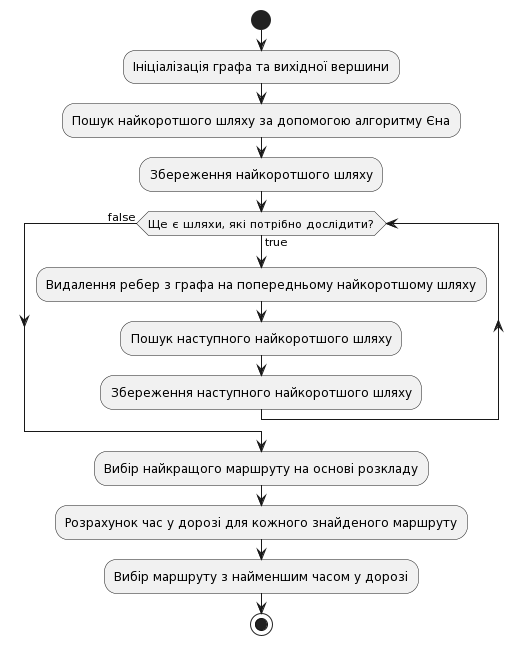
\includegraphics[scale=0.6]{content/chapters/2-implementation-methods/assets/img/timed_search_algorithm.png}
    \caption{Блок-схема алгоритму пошуку маршруту з урахуванням розкладу руху}
    \label{fig:timed_search}
\end{figure}

% \subsection{Потреби індивідуальних користувачів}
\label{subsec:individual-users-needs}

Для більш дотального розуміння потреб індивідуальних користувачів слід 
розглянути групи людей, які користуються громадським транспортом:\\

	Люди, які їздять на роботу

    Люди, які їздять на роботу, є одними з основних користувачів громадського транспорту. Їм потрібна можливість швидко і легко знаходити найкоротші та найшвидші маршрути до місця призначення. Крім того, їм може знадобитися зберігати часто використовувані маршрути.\\

    Туристи

    Туристи є ще однією ключовою групою користувачів. Вони можуть бути не знайомі з системою громадського транспорту в новому місті і потребують можливості швидко і легко знаходити найкращі маршрути до популярних туристичних місць. Крім того, вони можуть захотіти зберегти свої маршрути для подальшого використання або поділитися ними з друзями та родиною.\\

    Студенти та школярі

    Студенти та школярі також значною мірою покладаються на громадський транспорт, щоб дістатися до школи чи університету. Їм потрібно вміти знаходити найшвидші та найкоротші маршрути до кампусу та додому. Їм також може знадобитися планувати свої маршрути з урахуванням розкладу занять або інших зобов'язань, таких як позакласні заходи або робота з неповним робочим днем.\\

	Ділові мандрівники

	Діловим мандрівникам часто потрібно дістатися до місця призначення якомога швидше. Вони повинні мати можливість знайти найшвидший і найефективніший маршрут, беручи до уваги трафік, розклад громадського транспорту та інші фактори.


Загалом, користувачі послуг маршрутизації громадського транспорту потребують точної та актуальної інформації про розклад та маршрути. Їм також потрібен зручний інтерфейс, який дозволяє швидко і легко знаходити потрібну інформацію. Іншими важливими функціями є можливість зберігати маршрути та ділитися ними, інформування в режимі реального часу про збої та затримки.
